\documentclass[10pt,a4paper,onecolumn]{article}
\usepackage[utf8]{inputenc}
\usepackage[francais]{babel}
\usepackage[margin=2cm]{geometry}
\usepackage[T1]{fontenc}
\usepackage{amsmath}
\usepackage{amsfonts}
\usepackage{amssymb}
\usepackage{listings}
\usepackage{graphicx}

\lstset{
  language=Python,
  showstringspaces=false,
  formfeed=newpage,
  tabsize=4,
  commentstyle=itshape,
  morekeywords={models, lambda, forms}
}

\author{Fabien PETITJEAN}
\title{E571. Un joli tour de cartes}

\begin{document}
\maketitle
\begin{abstract}
Puce informe le public que Zig, pour le moment dans sa loge, va dans quelques instants réaliser un véritable tour de magie avec un jeu de 32 cartes.
Dans un premier temps, Puce convainc le public que les cartes ne sont ni biseautées ni truquées puis il décrit le déroulement du tour de cartes en ces termes :
{\it
\begin{itemize}
\item Le public choisira une carte (désignée par X) dont je prendrai connaissance.
\item Un premier volontaire dans la salle viendra mélanger les 32 cartes autant de fois qu’il le désire avant de les étaler sur une table en quatre rangées de huit cartes, faces cachées.
\item Un deuxième volontaire choisira à sa convenance un nombre de cartes qu’il retournera faces visibles.
\item A mon tour, je retournerai {\bf une seule} carte, qu’elle soit face visible ou face invisible.
\item Je quitterai la scène avant l’arrivée de Zig et j’irai au fond de la salle afin qu’on ne puisse pas me soupçonner de communiquer une quelconque information à mon partenaire.
\item Zig arrivera sur scène et au bout de quelques secondes annoncera à voix forte le nom de la carte X. S’il dit juste, vous êtes invités à l’applaudir chaleureusement.
\end{itemize}
}


\vspace{6mm}\noindent L'énoncé complet peut être trouvé sur le site {\tt http://diophante.fr}.
\end{abstract}

\section{Solution}
Puce et Zig se mettent d'accord sur ceci : chaque carte du jeu est associé à un nombre compris entre 0 et 31 de façon bijective. Pour trouver la valeur associée à une configuration de cartes données, on procède ainsi : on note en colonne le numéro de position (en base 2) de chaque carte qui est face visible. On a donc 5 colonnes et autant de lignes que de cartes faces visibles.
En bas de chaque colonne, on inscrit un 0 s'il y a un nombre pair de 1 dans la colonne et un 1 dans le cas contraire. Ces 5 nouveaux chiffres donnent un nombre en base 2 que l'on reconvertit en base 10 pour obtenir la valeur associé à la configuration.

Si on prend l'exemple donné sur le site {\tt http://diophante.fr}, on a les cartes 0, 1, 4, 7, 10, 11, 14, 15, 16, 18, 20, 27 et 29 qui ont leur face visible, cela donne le tableau suivant :

\begin{tabular}{|c|c|c|}
\hline
0  & 00000 & \it 00000 \\
1  & 00001 & \it 00001 \\
4  & 00100 & \it 00101 \\
7  & 00111 & \it 00010 \\
10 & 01010 & \it 01000 \\
11 & 01011 & \it 00011 \\
14 & 01110 & \it 01101 \\
15 & 01111 & \it 00010 \\
16 & 10000 & \it 10010 \\
18 & 10010 & \it 00000 \\
20 & 10100 & \it 10100 \\
27 & 11011 & \it 01111 \\
29 & 11101 & \it 10010 \\\hline
18 & 10010 &  \\\hline
\end{tabular}

La troisième colonne montre que l'on peut faire le calcul au fur et à mesure, évitant ainsi de devoir mémoriser toutes la colonne. Cela demande tout de même une bonne force de calcul mental, mais on peut s'aider avec les doigts. Pour mémoriser un nombre binaire de 5 bits, il suffit de mettre une main dans sa poche et d'affecter un bit à chaque doigt. Si le doigt touche la cuisse, c'est un 0, s'il est relevé, c'est un 1.

C'est tout ce que Zig doit savoir.

\vspace{8cm}
Pour Puce c'est plus dur puisqu'il doit aussi savoir comment passer d'un nombre quelconque à un autre nombre quelconque en ne retournant qu'une seule carte.
Il doit comparer les représentations en base 2 de la valeur actuellement affichée sur la table et de la valeur qu'il veut que la table affiche. A chaque fois qu'un bit diffère, il note 1 (mentalement), sinon il note 0. Le nombre résultant est le numéro de la carte qu'il doit retourner.

Supposons qu'on ait sur la table une configuration dont la valeur est {\bf 10010}. Puce veut coder le nombre 21 dont la représentation binaire est {\bf 10101}. Seuls les 3 derniers bits sont différents, cela donne le nombre {\bf 00111} qui vaut 7 en base 10. Puce doit donc retourner la carte {\bf 7}.

\section{Explication}
Je vais tenter d'expliquer comment j'en suis arrivé à cette solution.
Comme dans toute recherche, il y a des hypothèses qui nous font suivre de fausses pistes pendant des jours. Je vous ferai grâce de ces fourvoiements en ne détaillant que ce qui m'a permis de progresser vers la solution présentée ci-dessus.

\subsection{L'information cachée}
Ce qui semble sur, c'est que Puce communique avec Zig en modifiant la configuration du jeu de carte étalé sur la table. Il doit y avoir un code qui permette de trouver un nombre de 0 à 31 en fonction de quelle carte est face cachée et quelle carte est face visible. On fait l'hypothèse qu'il s'agit d'un code binaire qui ne se préoccupe pas de ce que montre la carte, mais seulement de son état caché ($0$) ou visible ($1$).

Il faut donc trouver un code qui permette de transformer un nombre de 32 bits en nombre entier compris entre 0 et 31, c'est-à-dire en un nombre à 5 bits.

Mais il faut en plus respecter une contrainte très ... contraignante :

\par\noindent\hrulefill\par
{\large
Si on prend un nombre à 32 bits quelconque $N$, on peut créer 32 nombres à 32 bits $N_i$ en inversant le bit $i\in [0..31]$. Alors le décodage de tous ces $N_i$ donne 32 nombres distincts compris entre 0 et 31.
}
\par\noindent\hrulefill\par

En effet, quand un volontaire va retourner au hasard certaines cartes sur la table, il va créer un nombre qui va se décoder en $17$, par exemple. Mais si Puce veut faire découvrir $23$ en retournant une seule carte, il faut que le système le permette.

C'est évidemment là que repose toute la difficulté.

\subsection{Étude d'un jeu de 4 cartes}
J'ai d'abord essayé de trouver une solution avec un jeu ne comportant que 4 cartes. Et après quelques tâtonnements, j'ai obtenu le diagramme symétrique suivant :

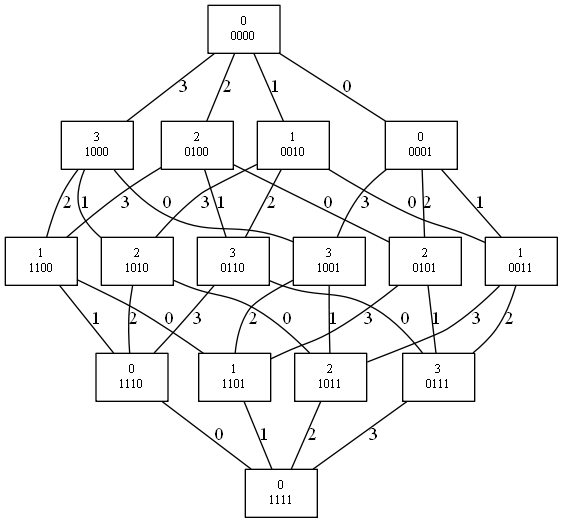
\includegraphics[width=16cm,keepaspectratio]{order4.png}

Dans chaque rectangle sont indiquées la configuration des 4 cartes (1 pour face visible et 0 pour face cachée) et la valeur associée. Les lignes relient des configurations qui se déduisent l'une de l'autre par retournement d'une seule carte. Les nombres inscrits sur ces lignes indiquent la différence en valeur absolue entre les valeur des deux configurations reliées.

On remarque deux choses :
\begin{itemize}
\item si on retourne toutes les cartes, on obtient la même valeur,
\item et si on retourne uniquement le dernier bit (le plus à droite) également.
\end{itemize}

\subsection{Étude d'une jeu de 8 cartes}
Pour pouvoir étudier des jeux de cartes avec plus de 4 cartes, j'ai trouvé plus facile d'utiliser l'ordinateur pour générer de tels graphes. % Je donne en annexe l'algorithme (codé en Javascript) qui permet de trouver un graphe à partir d'un nombre de cartes.

Je remarque alors que l'algorithme ne trouve aucune solution lorsque le nombre de cartes n'est pas un multiple de 2.

Le dessin du premier autre graphe possible comporte $2^8 = 256$ configurations, avec 8 lignes partant de chacune d'elles : il est illisible, mais je peux dresser un tableau des configurations en fonction de leurs valeurs.

\begin{tabular}{|c|c|c|c|c|c|c|c|}
\hline
\bf 0 & \bf 1 & \bf 2 & \bf 3 & \bf 4 & \bf 5 & \bf 6 & \bf 7 \\ \hline
00000000 & 00000010 & 00000100 & 00000110 & 00010000 & 00010010 & 00010100 & 00010110 \\
00000001 & 00000011 & 00000101 & 00000111 & 00010001 & 00010011 & 00010101 & 00010111 \\
00001110 & 00001100 & 00001010 & 00001000 & 00011110 & 00011100 & 00011010 & 00011000 \\
00001111 & 00001101 & 00001011 & 00001001 & 00011111 & 00011101 & 00011011 & 00011001 \\
00110010 & 00110000 & 00110110 & 00110100 & 00100010 & 00100000 & 00100110 & 00100100 \\
00110011 & 00110001 & 00110111 & 00110101 & 00100011 & 00100001 & 00100111 & 00100101 \\
00111100 & 00111110 & 00111000 & 00111010 & 00101100 & 00101110 & 00101000 & 00101010 \\
00111101 & 00111111 & 00111001 & 00111011 & 00101101 & 00101111 & 00101001 & 00101011 \\
01010100 & 01010110 & 01010000 & 01010010 & 01000100 & 01000110 & 01000000 & 01000010 \\
01010101 & 01010111 & 01010001 & 01010011 & 01000101 & 01000111 & 01000001 & 01000011 \\
01011010 & 01011000 & 01011110 & 01011100 & 01001010 & 01001000 & 01001110 & 01001100 \\
01011011 & 01011001 & 01011111 & 01011101 & 01001011 & 01001001 & 01001111 & 01001101 \\
01100110 & 01100100 & 01100010 & 01100000 & 01110110 & 01110100 & 01110010 & 01110000 \\
01100111 & 01100101 & 01100011 & 01100001 & 01110111 & 01110101 & 01110011 & 01110001 \\
01101000 & 01101010 & 01101100 & 01101110 & 01111000 & 01111010 & 01111100 & 01111110 \\
01101001 & 01101011 & 01101101 & 01101111 & 01111001 & 01111011 & 01111101 & 01111111 \\
10010110 & 10010100 & 10010010 & 10010000 & 10000110 & 10000100 & 10000010 & 10000000 \\
10010111 & 10010101 & 10010011 & 10010001 & 10000111 & 10000101 & 10000011 & 10000001 \\
10011000 & 10011010 & 10011100 & 10011110 & 10001000 & 10001010 & 10001100 & 10001110 \\
10011001 & 10011011 & 10011101 & 10011111 & 10001001 & 10001011 & 10001101 & 10001111 \\
10100100 & 10100110 & 10100000 & 10100010 & 10110100 & 10110110 & 10110000 & 10110010 \\
10100101 & 10100111 & 10100001 & 10100011 & 10110101 & 10110111 & 10110001 & 10110011 \\
10101010 & 10101000 & 10101110 & 10101100 & 10111010 & 10111000 & 10111110 & 10111100 \\
10101011 & 10101001 & 10101111 & 10101101 & 10111011 & 10111001 & 10111111 & 10111101 \\
11000010 & 11000000 & 11000110 & 11000100 & 11010010 & 11010000 & 11010110 & 11010100 \\
11000011 & 11000001 & 11000111 & 11000101 & 11010011 & 11010001 & 11010111 & 11010101 \\
11001100 & 11001110 & 11001000 & 11001010 & 11011100 & 11011110 & 11011000 & 11011010 \\
11001101 & 11001111 & 11001001 & 11001011 & 11011101 & 11011111 & 11011001 & 11011011 \\
11110000 & 11110010 & 11110100 & 11110110 & 11100000 & 11100010 & 11100100 & 11100110 \\
11110001 & 11110011 & 11110101 & 11110111 & 11100001 & 11100011 & 11100101 & 11100111 \\
11111110 & 11111100 & 11111010 & 11111000 & 11101110 & 11101100 & 11101010 & 11101000 \\
11111111 & 11111101 & 11111011 & 11111001 & 11101111 & 11101101 & 11101011 & 11101001 \\
\hline
\end{tabular}

Les remarques pour le jeu à 4 cartes sont aussi valable ici, alors on peut se limiter aux 6 bits centraux dans chaque configuration. En effet, si le premier bit est un 1, il suffit d'inverser tous les autres pour se retrouver dans une situation connue. Et comme le dernier ne change pas la valeur, notre fonction de codage ne va pas s'en servir non plus.

On obtient alors le tableau suivant : 

\begin{tabular}{|c|c|c|c|c|c|c|c|}
\hline
\bf 0 & \bf 1 & \bf 2 & \bf 3 & \bf 4 & \bf 5 & \bf 6 & \bf 7 \\ \hline
000000 & 000001 & 000010 & 000011 & 001000 & 001001 & 001010 & 001011 \\
000111 & 000110 & 000101 & 000100 & 001111 & 001110 & 001101 & 001100 \\
011001 & 011000 & 011011 & 011010 & 010001 & 010000 & 010011 & 010010 \\
011110 & 011111 & 011100 & 011101 & 010110 & 010111 & 010100 & 010101 \\
101010 & 101011 & 101000 & 101001 & 100010 & 100011 & 100000 & 100001 \\
101101 & 101100 & 101111 & 101110 & 100101 & 100100 & 100111 & 100110 \\
110011 & 110010 & 110001 & 110000 & 111011 & 111010 & 111001 & 111000 \\
110100 & 110101 & 110110 & 110111 & 111100 & 111101 & 111110 & 111111 \\
\hline
\end{tabular}


Voilà, il ne me reste plus qu'à trouver un codage qui permette de transformer tout nombre d'un colonne donnée par la valeur inscrite en en-tête. Cette valeur comprise entre 0 et 7 s'écrit en binaire à l'aide de 3 bits.

Je fais de nombreux essais, mais je ne trouve rien. Il faut dire que comme j'avais trouvé ce problème sur le site {\tt diophante.fr},  j'ai tout de suite pensé à utiliser l’arithmétique modulaire. Mais finalement, cette histoire de bits m'a rappelé que j'étais un informaticien et j'ai donc utilisé des outils qui me sont plus familiers : les opérateurs binaires AND, OR et XOR.

J'ai écrit différents programmes pour tester des assemblages de ces opérateurs et finalement l'un d'eux ma donné la solution.

Le code générique que je recherchais est le suivant :
{\tt
J'initialise la variable $v$ à $0$.\\
Pour chaque $b$ de 1 à 6:\\
\hspace{8mm}Si le bit $b$ de ma configuration vaut $1$:\\
\hspace{16mm}Assigner à $v$ le résultat de $v\text{XOR}N_b$.
\hspace{8mm}Fin Si\\
Fin Pour\\
}
Le tout est de trouver les $N_b$. Il y a $7^6= 117649$ possibilités : un jeu d'enfant pour un ordinateur.

Quel ne fut ma surprise de trouver la simple formule suivante : $N_b = b$. Ça parait tellement simple que j'aurais du le trouver à la main.

\subsection{Vérification}
Démontrons que notre méthode fonctionne.

Pour cela, il faut se pencher sur l'opérateur XOR (que l'on notera $.$ dans la suite) dont voici la table de vérité :

\begin{tabular}{|c|c|c|}
\hline
$A$ & $B$ & $A.B$ \\\hline
0 & 0 & \bf 0 \\\hline
0 & 1 & \bf 1 \\\hline
1 & 0 & \bf 1 \\\hline
1 & 1 & \bf 0 \\\hline
\end{tabular}

Sans rentrer dans le détail des démonstrations, voici les propriétés intéressantes du XOR :
\begin{itemize}
\item $\forall n, n.0 = 0.n = n$
\item $\forall n, n.n = 0$
\item $\forall (a,b), a.b = b.a$
\item $\forall (a,b,n), a.n = b \iff a.n.n = b.n \iff a = b.n$
\end{itemize}


Appelons \emph{configuration} une séquence de 32 cartes dont certaines sont face cachée (on les notera 0) et d'autres faces visibles (on les notera 1).

Appelons \emph{valeur d'une configuration} un nombre de $[0..31]$ obtenu en appliquant des XOR entre tous les index des cartes faces visibles de la configuration.

Appelons \emph{voisin d'une configuration} une configuration obtenue en retournant une seule carte à la configuration initiale.

Appelons \emph{voisinage d'une configuration} l'ensemble des voisins de cette configuration.

Si $v$ est la valeur d'une configuration, alors son voisinage est l'ensemble suivant :
$\{v.i \;\text{ tel que }\; i\in [0..31]\}$.

Si tous les $v.i$ sont distincts, l'ensemble a un cardinale de 32 donc notre méthode permet de passer d'une valeur quelconque à une autre valeur quelconque en ne retournant qu'une seule carte.

Prouvons que les $v.i$ sont distincts par l'absurde. Soit $i\neq j$ tels que $v.i = v.j$, alors il existe un $x$ tel que $v.i = x = v.j$. On a donc $v.v.i = v.x = v.v.j$ qui équivaut à $i = v.x = j$. Cela contredit $i\neq j$.



\end{document}